% This is samplepaper.tex, a sample chapter demonstrating the
% LLNCS macro package for Springer Computer Science proceedings;
% Version 2.20 of 2017/10/04
%
\documentclass[runningheads]{llncs}
%
\usepackage{graphicx}
\usepackage[utf8]{inputenc}
\usepackage{subfig}
% Used for displaying a sample figure. If possible, figure files should
% be included in EPS format.
%
% If you use the hyperref package, please uncomment the following line
% to display URLs in blue roman font according to Springer's eBook style:
% \renewcommand\UrlFont{\color{blue}\rmfamily}

\begin{document}
%
\title{Versinus: an Animated Visualization Method for Dynamic Scale-Free Networks\thanks{Supported by FAPESP, project 2017/05838-3}}
%
%\titlerunning{Abbreviated paper title}
% If the paper title is too long for the running head, you can set
% an abbreviated paper title here
%
\author{Renato Fabbri\orcidID{0000-0002-9699-629X} \and
Maria Cristina Ferreira de Oliveira\orcidID{0000-0002-4729-5104}}
%
\authorrunning{R. Fabbri and M. C. F. de Oliveira}
% First names are abbreviated in the running head.
% If there are more than two authors, 'et al.' is used.
%
\institute{University of São Paulo, São Carlos SP, Brazil\\
\email{renato.fabbri@gmail.com},
\email{cristina@icmc.usp.br}}
%\url{http://conteudo.icmc.usp.br/pessoas/cristina/}}
%
\maketitle              % typeset the header of the contribution
%
\begin{abstract}
% The abstract should briefly summarize the contents of the paper in
% 150--250 words.
Most real-world networks are dynamic, i.e., they change over time as nodes and links are added or removed, and their representation may also involve variations in the associated data.
There is a growing interest in modeling dynamic (or time-evolving, or longitudinal) networks and
a number of procedures have been proposed to visualize them.
  This article presents a visualization method for dynamic scale-free networks.
  Compliant methods were not found in other tools by the authors, which motivated this description and the development of a dedicated interface.
  Named Versinus, the visualization is specially useful in the observation of (in)stability of basic topological characteristics, and consists essentially in placing the most connected nodes (hubs and intermediary) along a sine curve, and the peripheral nodes along a separate segment, usually a line.
  Thus its name, from  Latin \emph{versus} (line) and \emph{sinus} (sine).
  The Versinus visualization can provide insight into network properties and is useful for observing its behavior, as described in this paper, after a formal presentation of the method and its associated software implementations.
\keywords{Network visualization
\and Dynamic networks
\and Longitudinal networks
\and Time-evolving networks
\and Evolving networks
\and Animated visualization
\and Complex networks
\and Data visualization.}
\end{abstract}
%
%
%
\section{Introduction}
The visualization of dynamic networks poses challenges related to data size and complexity which have merited various contributions~\cite{evo1,hajij,evo3,evo2}.
In fact, the meaningful visualization of dynamic networks is a well-known problem in Information Visualization and dynamic network analysis.
In this work, we present an approach for dynamic network visualization that consists in distributing the nodes along a fixed layout arranged in three segments associated with the three sectors (or partitions) of a scale-free network, namely for the hub, intermediary and peripheral nodes~\cite{stab}. The network dynamic features are expressed by means of changes in visual properties of the glyphs used to depict nodes and links, e.g., glyph height, width, color and shape, and line (arrow) disposition, thickness and color. Moreover, complementary global and local information is rendered in order to enable an acoustic depiction of features of interest.
The method has been called Versinus since its early usages in 2013, because the layout stabilized, after attempts with distinct arrangements, in a sine period and a line, which in Latin is \emph{sinus} (sine) and \emph{versus} (line). 
There are four software implementations of Versinus, two of them written in Python scripts and packages that yield animations through stop-motion. The other two are written in JavaScript, one focused on exploitation of static networks, the other is an experimental Visual Analytics interface, which extends the visual metaphor to the 3D space and provides additional analysis techniques such as principal component analysis (PCA) and resources for structure navigation\footnote{An instance of the interface is available at: http://rfabbri.vicg.icmc.usp.br:3000/evolution}.
The writing of this document was motivated by
the fact that no method was found by the authors that aims at visualizing dynamic scale-free networks through node-link diagrams.
Furthermore, the visualization method was employed in scientific research~\cite{thesis,stab}, and thus a careful mathematical and technological description of the procedures involved in applying Versinus to real networks is appropriate.

The article is organized as follows. The next subsections address related work and issues of nomenclature. Section~\ref{sec:des} describes the method in detail and sufficient formalism. Section~\ref{sec:imp} outlines the software implementations of Versinus and depicts the resulting animations. Section~\ref{sec:ins} is dedicated to revealing further insights obtained through the use of the method. Finally, Section~\ref{sec:con} assembles concluding commentaries and further work.

\subsection{Related work}
% on animated visualization
% on vis of evo nets
Although animation for the purposes of data analysis is often criticized in the data visualization literature, advantages have also been reported~\cite{anim,munzner,cog,ware}, e.g.: yielding visualizations more eye catching and taking advantage of the fact that humans are used to interacting with moving objects.
Dynamic network visualization has been tackled both through animated and static (often timeline-based) visualizations~\cite{hajij,brain,visAn,ego}, focusing on various global and local network features.
The contribution reported in this document is singular in that it consists basically of a layout which is fit for networks with scale-free characteristics, in association with some visualization cues which are implementation dependent. It results from extensive attempts to reach a satisfactory visualization by means theoretical and intuitive strategies and methodical verification of the result by appreciation of the entailed animations.
The procedures and conceptualizations involved in achieving the final visualization were also considered worth documenting, as they were not found elsewhere in the literature, and by virtue of the simple and genuine design. Its scientific relevance on a practical application has been demonstrated before~\cite{stab}.

\subsection{Remarks on nomenclature}
Dynamic networks are also called e.g. longitudinal networks, time-evolving networks, evolving networks, and time-varying networks~\cite{ev,tev,tv,lg}.
We chose to adopt the term ``dynamic network'' herein because it is simple, semantically meaningful and has been widely adopted.
Another major issue in current vocabulary is in the phrase ``sector of a network'' (e.g. of the hubs). In most cases, the sectors are also partitions (i.e. they are non-overlapping sets whose union is the complete superset), but it depends on the criteria for obtaining the sectors~\cite{stab}, thus the use of the more general term \emph{sector}.
Moreover, network science is highly multidisciplinary and context-dependent, and flourished from the ill-defined area of complex systems, favoring polysemy and synonymy. We strove to avoid such issues and keep a consistent usage of nomenclature.
%because they are usually not convenient in scientific literature.

\section{A description of the method}\label{sec:des}
Versinus generates a layout through placing the nodes in segments
with respect to their overall topological features and then representing
instantaneous topological features though glyph and arrow attributes.
The visualization may be thus split in three stages, described in the following subsections.

\subsection{Node placement}\label{sec:pla}
First, a network is constructed with all the activity of interest, i.e. the transactions such as all the email messages considered, or all the links in a data file.
The nodes are then ordered either by degree or strength (or in- or out-degree or strength), from greatest to smallest values.
Also from such global network, the hubs, intermediary and peripheral sectors are obtained. Two methods have been proven useful for obtaining sectors: 1) assuming fixed fractions of hubs (e.g. 5\%), of intermediary (e.g. 15\%) and peripheral nodes (e.g. 80\%); 2) by comparison of the network against the Erdös-Rényi model, a non-trivial procedure, with relevant analytical results, detailed elsewhere~\cite{stab}.

With such structures at hand, the nodes are placed along three segments, as depicted in Figure~\ref{fig:glob}.
The hubs are placed along the first half of a sine period.
The intermediary nodes are placed along the second half of the sine period.
The peripheral nodes are placed along an independent line.
The placement follows 
the basic parameters:
\begin{itemize}
  \item The amplitude $\alpha$ of the sine oscillation.
  \item The displacement $\Delta$ of the sine in the vertical axis.
  \item The horizontal margin $\mu$, i.e. the distance from the left border to the first hubs, assumed the same as the distance from the right border to last intermediary node.
  \item The positions $(x_0,y_0)$ and $(x_1,y_1)$, i.e. the endpoints of the segment for the peripheral sector.
\end{itemize}

\begin{figure}[!h]\centering
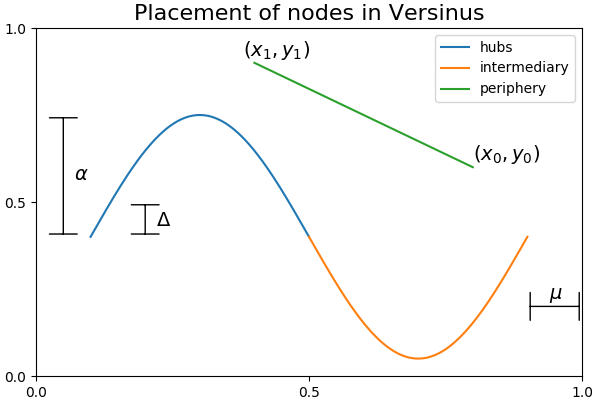
\includegraphics[width=.7\textwidth]{nodePositioning}
  \caption{The underlying layout of Versinus. Highly connected nodes are positioned from left to right on the sine segment (for the hubs and intermediary sectors), and from right to left on the upper line (for the periphery sector). The parameters are: amplitude $\alpha$ of the oscillation; vertical displacement $\Delta$ of the oscillation; horizontal margin $\mu$; and line endpoints $(x_0, y_0)$ and $(x_1, y_1)$.
   Further information is given in Section~\ref{sec:pla}.
  }\label{fig:glob}
\end{figure}

\noindent Some crafty remarks: fine-tuning the size (number of nodes) of each sector may come handy due to the node density and activity in each segment. Also, the node placed at the middle of the sine period may be a hub or an intermediary node, and this choice often impacts the clarity of the final visualization more than anticipated by intuition.
Finally, avoiding clutter with the hubs motivated both 
the positioning of the peripheral sector in the upper-right corner and
the placement of the most active peripheral nodes next to the intermediary sector, i.e. the ordering along the peripheral line.

\subsection{Drawing nodes, links and auxiliary information}
Additional concepts and quantities need to be defined for visualizing the evolving network as a data-driven animation.
A \emph{snapshot} $S$ consists of a number $\sigma$ time-contiguous transactions, e.g. 100 email messages, starting at an arbitrary message.
The separation $\eta$ between each snapshot is the number of transactions skipped from one snapshot to the next.
In summary, the evolving network is visualized through a sliding window of $\sigma$ transactions, updated at every $\eta$ transactions. To achieve the final animation, a transaction rate $\omega$ must also be defined.
Thus, the following parameters are specified:
\begin{itemize}
  \item The window $\sigma$ captured at each snapshot, expressed in transactions.
  \item The step size $\eta$ between each snapshot, expressed in transactions.
  \item The transaction rate $\omega$, expressed in transactions per second.
\end{itemize}

\noindent The sequence of snapshots may be expressed as $\{S_i^{\sigma, \eta}\}_0^{L}$, where $L$ is the smallest integer such that $L\times \eta + \sigma > T$ and $T$ is the total number of transactions. Notice that the final snapshot $S_L$ may have less than $\sigma$ transactions. Also, the rate $\omega$ is only applied when rendering the animation, e.g. if each snapshot $S_i$ yields an image, the stop motion animation will use $\omega/\eta$ images per second to achieve the desired rate of $\omega$ transactions per second.

In each snapshot, the entailed network is analyzed in terms of the sectors (hubs, intermediary and periphery), in and out degree (or strength, if preferred) and clustering coefficient. Then the visual mapping of information is performed as follows:
\begin{itemize}
  \item Nodes not incident in the snapshot are not shown. Glyphs associated with nodes incident in the snapshot are assigned a minimum width and height.
  \item The node sector in the snapshot is mapped to a glyph shape (e.g. circle, hexagon and diamond for hub, intermediary and peripheral nodes, respectively).
  \item Node width is incremented proportionally to its in-degree (or out-strength, if preferred). Node height is incremented proportionally to its out-degree (or out-strength if preferred).
  \item Node color is related to clustering coefficient, e.g. zero is mapped to white, one is pure red, and intermediary values are scaled accordingly.
  \item Link weight is mapped to line width and/or a color scale.
\end{itemize}

\noindent Finally, complementary information may be displayed as a persistent legend that reveals essential information such as $\sigma$, $\eta$, $\omega$ and $T$, and keeps track of the current snapshot, e.g. its number of nodes and edges.
Also, node-specific information may be displayed by blinking corresponding cues over the nodes periodically, displaying them with a vertical displacement from the node, or by writing them to a specific widget when requested by the analyst on an interactive interface, i.e. on-demand.
Figure~\ref{fig:final} exemplifies two of the early flavors of Versinus settings.

\begin{figure}[!h]\centering
    \subfloat[]{{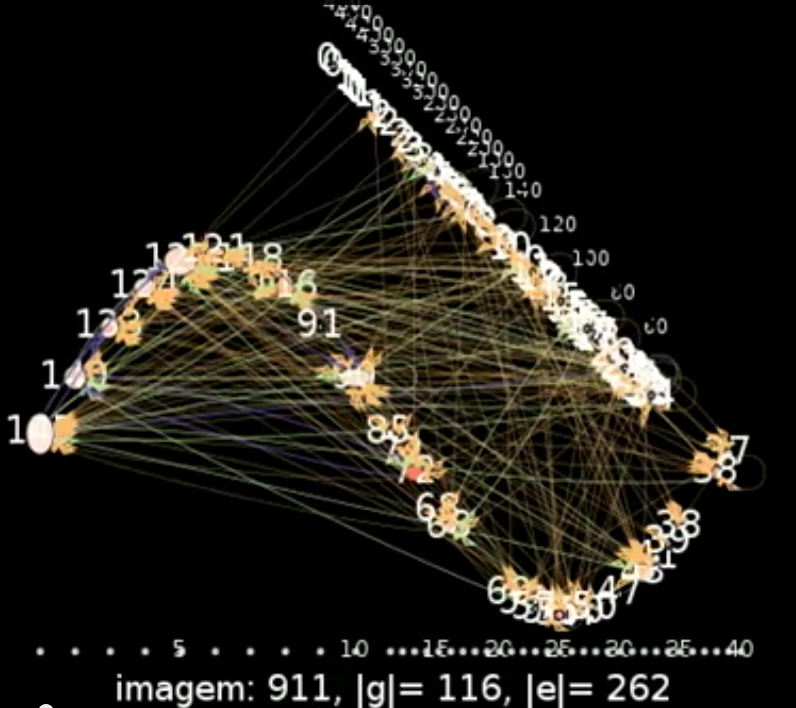
\includegraphics[width=.46\textwidth, height=4.3cm]{versinus_} }}%
    \quad
  \subfloat[]{{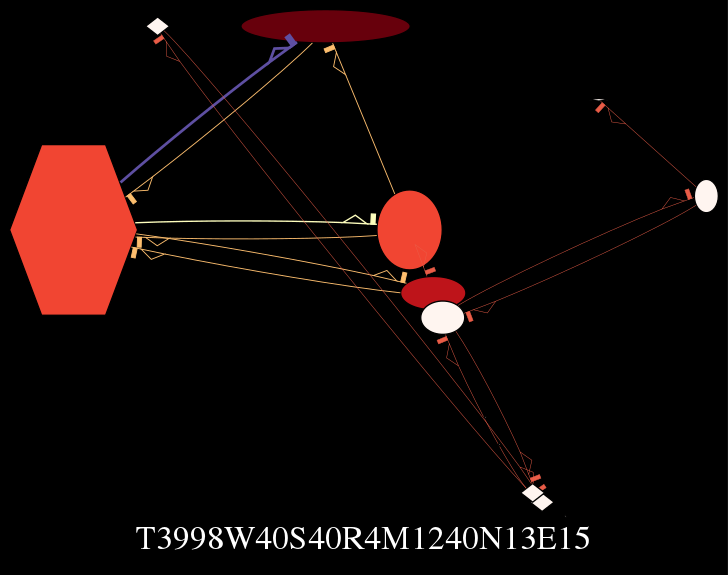
\includegraphics[width=.46\textwidth, height=4.3cm]{im31} }}%
    \caption{Two frames of dynamic network animations achieved using the Versinus method.
    Both are achieved through dedicated Python scripts and package modules.
    In (a) the individual degrees in the snapshot are blinking over the nodes, and the nodes are counted in auxiliary lines along the bottom and paralel to the periphery line. Current image/snapshot is 911 and has 116 nodes and 262 links.
   In (b), a cleaner version is employed to display a snapshot in which the only hub is the overall hub, the second overall hub is a peripheral node, and most nodes have high clustering coefficient. The legend indicates that the total number of transactions is $T=3,998$, the window size $\sigma=40$, the step size is $\eta=40$, the transaction rate is $\omega=4$, the current snapshot starts at transaction 1,240 and has 13 nodes and 15 links.
   The low-quality images are typical of the early implementations of Versinus, developed to assist the investigations of the researchers directly related to its development.
   Further information is given in Section~\ref{sec:des}.
   }%
    \label{fig:final}%
\end{figure}

\subsection{Observation of the evolving network}
Within the settings described, one may notice a number of network characteristics: do nodes (or a specific node) change their sectors often? Is the overall intermediary sector in greater activity with the hubs or periphery?
Does higher clustering really occur most often in the less connected nodes?
Are there very unbalanced nodes with respect to in and out degree (or strength)?
Is the number of nodes and edges stable along the network evolution?
In fact, Versinus was partly designed to inspect network attributes due to the remarkable stability of their overall characteristics reported in~\cite{stab}.
In this context, it is natural to ask if such stability is also noticeable in individual nodes or in connectivity patterns. Although the overall characteristics may be regarded as surprisingly stable, the stability of network components is very network-dependent. E.g.,  as suggested by~\cite{barabasiEvo}, all hubs were found to have intermittent activity in social networks, except for the smallest networks analyzed.

\section{Software implementations}\label{sec:imp}
Currently, there are four software implementations of Versinus known to the authors.
For organization and brevity, these are all linked in\footnote{Pivot repository for Versinus resources such as implementations, public instances of interactive interfaces, and videos: https://github.com/ttm/versinus}. 
Two of them are written in Python: one is a script that renders animations as in the Figure~\ref{fig:final}
(a), with more cues of local structure. The other is a library that renders animations as in the Figure~\ref{fig:final} (b), simpler and with more cues of the overall structure, and is capable of rendering sonifications of the dynamic networks, yielding ``audiovisualizations'', i.e. synced sonic and visual mappings of the dynamic networks.
The other two implementations are in JavaScript and use WebGL. One is, by default, for static (non-dynamic) networks, implemented as part of the ccNetViz library, that aims at being as computationally inexpensive as possible~\cite{cell}.
The other is an experimental 3D Visual Analytics application in which Versinus is combined with other analytical techniques,
such as principal component analysis, overview first - focus on demand, and simultaneous highlighting of corresponding structures across images as required by users.
These last two implementations are illustrated in Figure~\ref{fig:extra}.

\begin{figure}[!h]\centering
    \subfloat[Versinus in ccNetViz]{{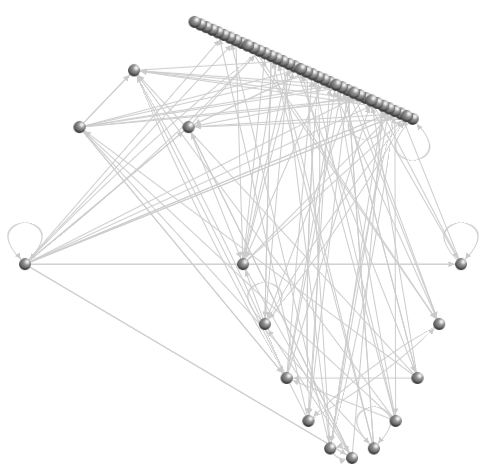
\includegraphics[width=.46\textwidth, height=2.5cm]{ccNetViz} }}%
    \qquad
  \subfloat[Experimental Visual Analytics]{{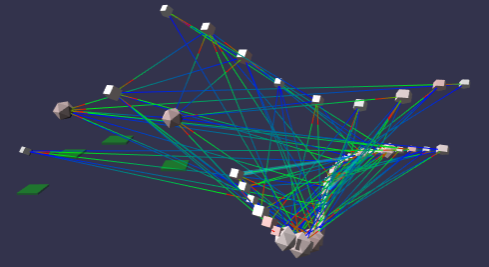
\includegraphics[width=.46\textwidth]{visAn} }}%
    \caption{Two implementations of Versinus in JavaScript using WebGL. (a) illustrates the implementation that is available within ccNetViz, a library purposed to being computationally inexpensive. This implementation handles static networks by default. (b) is an image achieved using an experimental Visual Analytics application.
    It renders the animations in real time, with multiple controls for inspecting the network structure and controlling the animation, in association with other analysis techniques. The sine oscillates both in the vertical and depth axes, as does the periphery segment. Further information is given in Section~\ref{sec:imp}.}
    \label{fig:extra}
\end{figure}

\subsection{Network sonification}\label{sson}
The implementation illustrated in Figure~\ref{fig:final} (b) includes a sonification routine for the evolving network.
Results are of limited effectiveness in the sense that the sonification does not enable users to grasp network features with ease,
specially if they are not musically trained.
Nevertheless, it made the (audio)visualization more engaging, as it yields exotic media,
and it is the first time the authors appreciated a sonification of an evolving network (maybe even of any network),
and is thus probably a unique multimedia representation of networks.
Accordingly, we understand suitable to provide a short description of the sonification as it was left implemented,
i.e. in its final version,
even though a full understanding of the summary requires knowledge of musical theory.
Four sonic/musical voices are used, two of them are noises and the other two have defined pitch. The lower noise has central frequency proportional to first hub connectivity,
which is the node positioned at the extreme left on the layout, on the starting point of the sine, and its frequency is updated every two beats.
The higher noise has central frequency proportional to the second hub, the node next to the first hub, and its frequency is updated at each beat.
The third hub connectivity is proportional to the lower note,
which is incident once a beat, and has its note value updated at every beat.
The fourth hub connectivity is proportional to the higher note, which is incident twice every half-beat, is updated at every note, and is only heard on the second half-beat of every tempo.
Figure~\ref{fson} illustrates such disposition of sonic lines (or musical voices).

\begin{figure}[!h]\centering
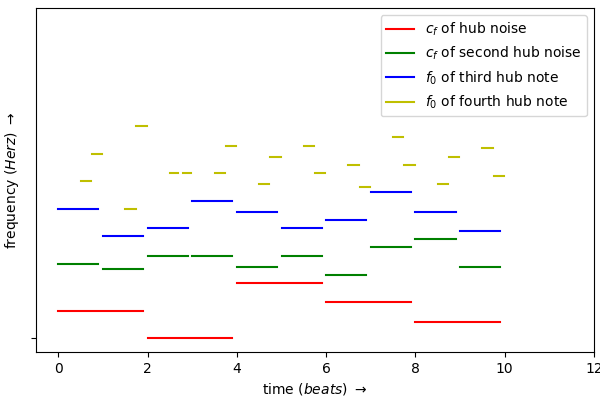
\includegraphics[width=.9\textwidth]{sonif}
  \caption{Visual representation of the sonification implemented for the dynamic networks.
  $c_f$ and $f_0$ stands for \emph{center frequency} and \emph{fundamental frequency}, respectively.
  Further details are given in Section~\ref{sson}.
  }\label{fson}
\end{figure}

\subsection{Animations produced and available}\label{sec:vid}
A number of animations were obtained through the routines described.
These encompassed different networks, settings ($\alpha$, $\sigma$, $\eta$,
etc), and different flavors of Versinus.
Some of these visualizations are available in six playlists of Youtube videos.
For organization and brevity, they are available at~\footnote{Pivot repository for Versinus resources such as implementations, public instances of interactive interfaces, and videos: https://github.com/ttm/versinus} together with other Versinus-related resources.

\subsection{An experimental Visual Analytics interface}
This section exemplifies the employment of the Versinus method
within a more elaborate framework.
Let us consider an interactive visual interface, with which the user may parametrize Versinus and then navigate through the entailed dynamic network.

\begin{figure}[!h]\centering
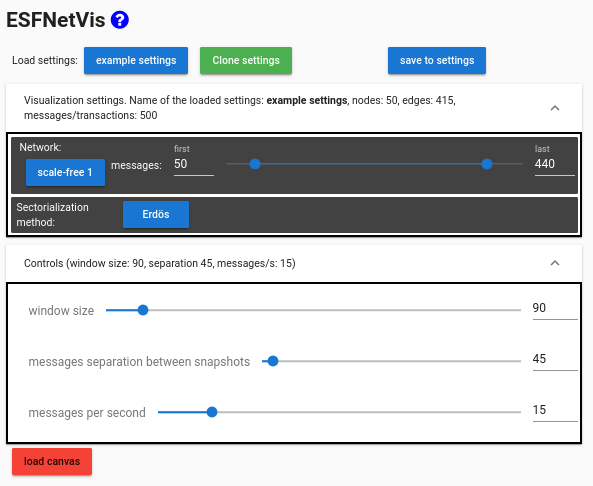
\includegraphics[width=\textwidth]{esfNetVis___}
  \caption{
  }\label{esfnetvis}
\end{figure}


\begin{figure}[!h]\centering
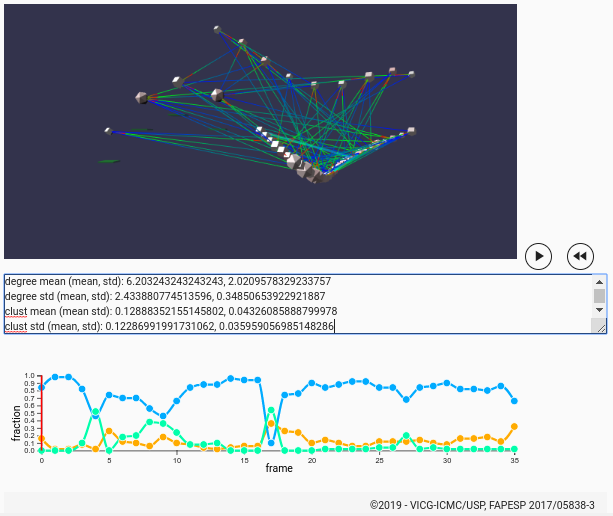
\includegraphics[width=\textwidth]{esfNetVis2___}
  \caption{
  }\label{esfnetvis}
\end{figure}

\begin{figure}[!h]\centering
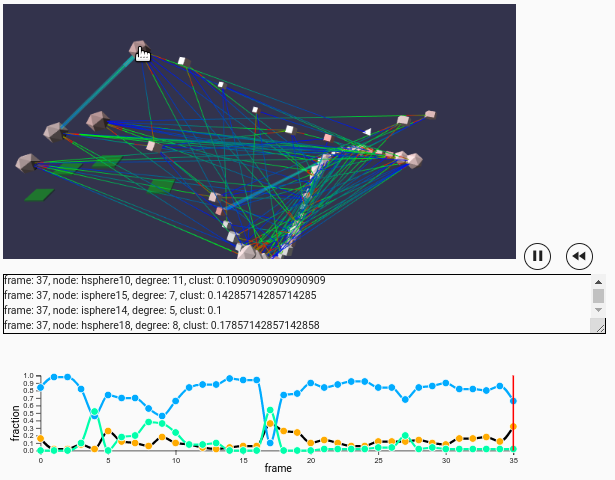
\includegraphics[width=\textwidth]{esfNetVis3}
  \caption{
  }\label{esfnetvis}
\end{figure}

\begin{figure}[!h]\centering
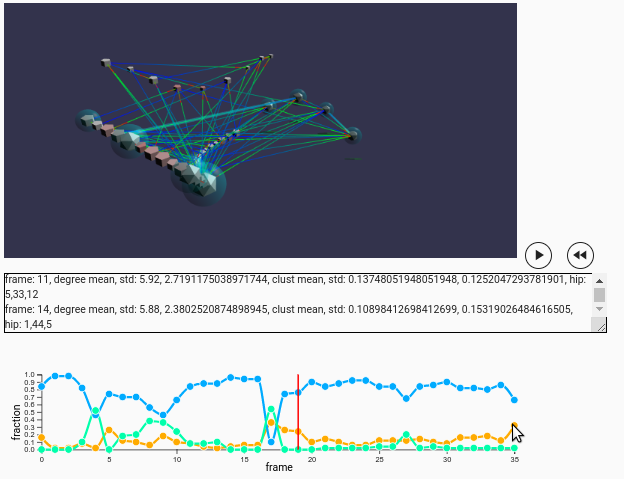
\includegraphics[width=\textwidth]{esfNetVis4}
  \caption{
  }\label{esfnetvis}
\end{figure}
One basic feature of the method is the constant representation of
nodes in each of the hubs, intermediary and peripheral sectors.
Nodes are positioned according to such classification regarding all
the activity of interest, and in each snapshot visual cues map the
classification within the snapshot.
Following the analytic methods used in~\cite{stab}, it may be crucial
to know how the relative sizes of the sectors vary along time, i.e. along
the sequence of snapshots.


\section{Insights gathered}\label{sec:ins}
This section describes insights gathered by the authors,
and should be further verified in subsequent work and using
suitable validation methods.
The legitimacy of the exposition herein given is based on the reasonable aspect of the assertions, and on the facts that the authors developed Versinus, used the method extensively, and the scientific contribution which it made possible~\cite{stab}.

The visualization of network structures is favored by the placement of nodes in an oscillatory pattern, as it tends to decrease the superposition of nodes and links. In fact, this principle was implemented in some of the layouts available within ccNetViz, and it may be useful in other well-known layouts, such as the Hive Plot~\cite{hive}.
Using a single period for the sine is an arbitrary choice, established because it entailed good visualizations for the networks and tasks at hand during the design of Versinus. Nonetheless, it is allowed to vary in more recent implementations in JavaScript\footnote{Pivot repository for Versinus resources such as implementations, public instances of interactive interfaces, and videos: https://github.com/ttm/versinus}: the sine in which the hub and intermediary nodes are positioned may have as many periods as parametrized by the analyst, and the same is feature is available for the segment for the peripheral nodes.
Another important insight is the pertinence of fixed positions for the observation of evolving networks.
Not only this has the potential to reduce the hairball effect~\cite{hairball},
but it is most often very difficult to keep track of individual nodes and structures when the nodes are allowed to move in the images while the network evolves, as in force-based layouts.
The placement of nodes with respect to their topological features (nodes are ordered by connectivity,
segments are related to network sectors) revealed very useful for understanding network features,
such as stability and connectivity-dependent behaviors.
Visual cues such as glyph width, height, shape and color were found informative for grasping information on individual nodes,
but results in a cognitive overload when attempting to observe global features,
which motivates simplified settings.
The sonification of the evolving network added to the exotic flavor of Versinus and made it more attractive.
However, it seems that more informative sonifications should require dedicated research,
training of already musically competent users, and very modest goals. 
Furthermore, reasonable parametrization (e.g. through $\alpha$, $\Delta$, $\mu$, $(x_0, y_0)$, $(x_1, y_1)$, $\sigma$, $\eta$ and $\omega$) is highly dependent on the network characteristics and user intended tasks, and calls for interactive interfaces and automated recommendation of initial values.

\section{Conclusions and further work}\label{sec:con}
This document presents a description of the Versinus visualization method, with its fundamental elements, usage potentials, and software implementations.
The validity of Versinus is implied both by its employment in published research~\cite{stab,thesis}, and the insights it yields on individual networks and network
layouts in general.
Further developments,
with focus on interactivity and Web technologies,
are currently being refined
through research and software development.

Next steps include
automated tuning of Versinus parameters, 
implementation of cues for relating language incident in the networks to their topology, and
further visually representing topological features (e.g. the fraction of interaction of the intermediary sector with the hubs and with the periphery).
The experimentation of Versinus features within other layouts is a potentially
valuable contribution, e.g. wiggling the segments of a Hive Plot~\cite{hive}.
We should implement further mechanisms for the detection of structural changes within the network evolution, such as using the persistent homology~\cite{hajij}.
Most importantly, we aim at completing a Visual Analytics utility to support using Versinus in an interactive environment for enhanced exploratory data analysis,
and verifying the claims described in Section~\ref{sec:ins} through formal validation techniques.
Finally, we plan to further analyze data sets of evolving networks~\cite{stab} using Versinus.


%
% ---- Bibliography ----
%
% BibTeX users should specify bibliography style 'splncs04'.
% References will then be sorted and formatted in the correct style.
%
\bibliographystyle{splncs04}
\bibliography{paperbib}
%
% \begin{thebibliography}{8}
% \bibitem{ref_article1}
% Author, F.: Article title. Journal \textbf{2}(5), 99--110 (2016)
% 
% \bibitem{ref_lncs1}
% Author, F., Author, S.: Title of a proceedings paper. In: Editor,
% F., Editor, S. (eds.) CONFERENCE 2016, LNCS, vol. 9999, pp. 1--13.
% Springer, Heidelberg (2016). \doi{10.10007/1234567890}
% 
% \bibitem{ref_book1}
% Author, F., Author, S., Author, T.: Book title. 2nd edn. Publisher,
% Location (1999)
% 
% \bibitem{ref_proc1}
% Author, A.-B.: Contribution title. In: 9th International Proceedings
% on Proceedings, pp. 1--2. Publisher, Location (2010)
% 
% \bibitem{ref_url1}
% LNCS Homepage, \url{http://www.springer.com/lncs}. Last accessed 4
% Oct 2017
% \end{thebibliography}
\end{document}
